% Equivalencia: convolucion espacial, grafo, filtro espectral
% Compilar con: pdflatex cnn_graph_kernel_spectral.tex
\documentclass[tikz,border=10pt]{standalone}
\usepackage{tikz}
\usepackage{pgfplots}
\pgfplotsset{compat=1.18}
\usepackage{amsmath,amssymb}

\usetikzlibrary{arrows.meta, positioning, calc, backgrounds}

\definecolor{gdlblue}{RGB}{41, 98, 168}
\definecolor{gdlred}{RGB}{191, 49, 49}
\definecolor{gdlgreen}{RGB}{30, 130, 76}
\definecolor{gdlorange}{RGB}{217, 130, 30}
\definecolor{gdlpurple}{RGB}{118, 56, 138}
\definecolor{gdlgray}{RGB}{140, 140, 140}
\definecolor{gdlyellow}{RGB}{190, 140, 10}

\begin{document}
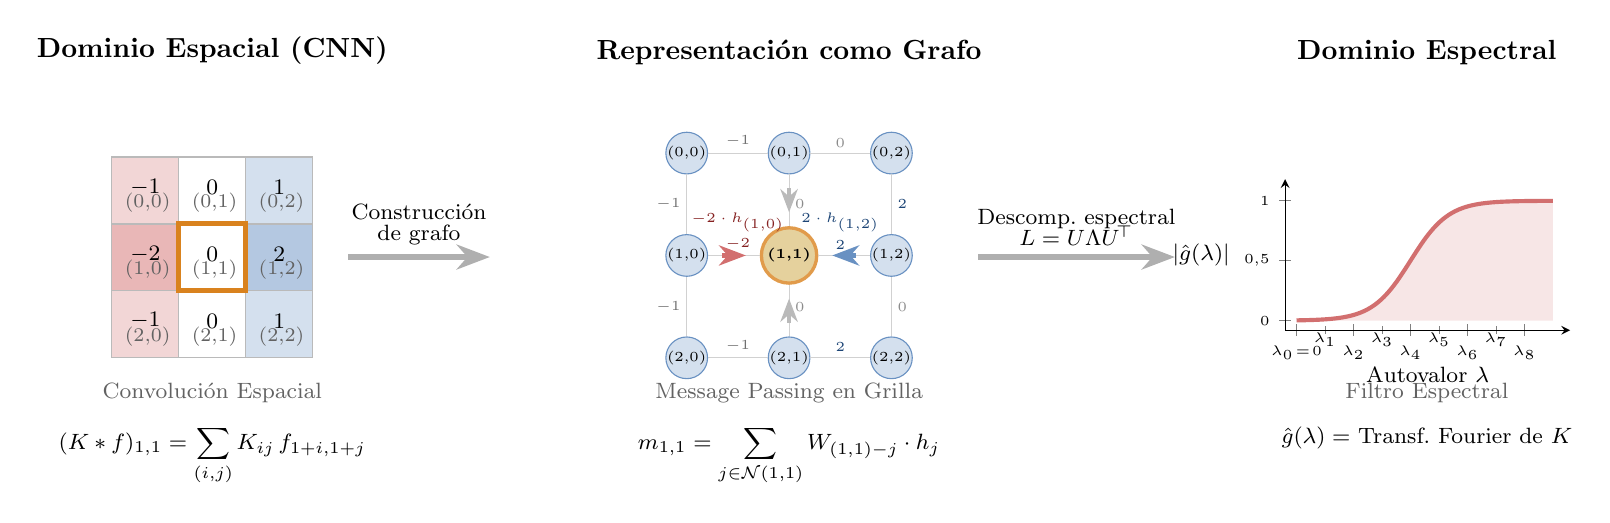
\begin{tikzpicture}[>=Stealth, font=\small]

% ============================================================
% Panel 1: Dominio Espacial (CNN) — Sobel kernel on 3x3 grid
% ============================================================
\begin{scope}[shift={(0,0)}]

    \node[font=\bfseries, anchor=south] at (1.275, 3.6) {Dominio Espacial (CNN)};

    \def\cellsize{0.85}

    % Draw cells with fill colors
    \foreach \r/\c/\val/\fillcol in {%
        0/0/-1/gdlred!20, 0/1/0/white, 0/2/1/gdlblue!20,
        1/0/-2/gdlred!35, 1/1/0/white, 1/2/2/gdlblue!35,
        2/0/-1/gdlred!20, 2/1/0/white, 2/2/1/gdlblue!20%
    }{%
        \pgfmathsetmacro{\xpos}{\c*\cellsize}
        \pgfmathsetmacro{\ypos}{(2-\r)*\cellsize}
        \fill[\fillcol] (\xpos, \ypos) rectangle +(\cellsize, \cellsize);
        \draw[gdlgray!60] (\xpos, \ypos) rectangle +(\cellsize, \cellsize);
        \node[font=\footnotesize\bfseries] at (\xpos+0.5*\cellsize, \ypos+0.55*\cellsize) {$\val$};
        \pgfmathtruncatemacro{\ri}{\r}
        \pgfmathtruncatemacro{\ci}{\c}
        \node[font=\tiny, text=gdlgray!70!black, anchor=south west]
            at (\xpos+0.04, \ypos+0.02) {\scriptsize(\ri,\ci)};
    }

    % Highlight center cell (1,1) with orange border
    \draw[gdlorange, thick, line width=1.8pt]
        (1*\cellsize, 1*\cellsize) rectangle +({\cellsize},{\cellsize});

    % Subtitle
    \node[font=\footnotesize, text=gdlgray!70!black, anchor=north] at (1.275, -0.2)
        {Convoluci\'{o}n Espacial};

    % Formula
    \node[font=\footnotesize, anchor=north] at (1.275, -0.75)
        {$(K * f)_{1,1} = \displaystyle\sum_{(i,j)} K_{ij}\, f_{1+i,1+j}$};
\end{scope}

% ============================================================
% Arrow 1: Left -> Middle
% ============================================================
\draw[->, line width=2pt, gdlgray!70]
    (3.0, 1.28) -- node[above, font=\footnotesize, text=black, align=center]
    {Construcci\'{o}n\\[-2pt]de grafo} (4.8, 1.28);

% ============================================================
% Panel 2: Representacion como Grafo
% ============================================================
\begin{scope}[shift={(7.3, 0)}]

    \node[font=\bfseries, anchor=south] at (1.3, 3.6) {Representaci\'{o}n como Grafo};

    % Node style
    \tikzset{
        gnode/.style={circle, draw=gdlblue!70, fill=gdlblue!20,
            minimum size=15pt, inner sep=0pt, font=\tiny},
        cnode/.style={circle, draw=gdlorange!80, fill=gdlyellow!40,
            minimum size=20pt, inner sep=0pt, font=\tiny\bfseries,
            line width=1.2pt}
    }

    \def\sep{1.3}
    % Place 3x3 nodes
    \foreach \r/\c in {0/0, 0/1, 0/2, 1/0, 1/2, 2/0, 2/1, 2/2}{
        \pgfmathsetmacro{\xp}{\c*\sep}
        \pgfmathsetmacro{\yp}{(2-\r)*\sep}
        \node[gnode] (n\r\c) at (\xp, \yp) {(\r,\c)};
    }
    % Center node
    \node[cnode] (n11) at (1*\sep, 1*\sep) {(1,1)};

    % 4-connectivity edges
    \foreach \ra/\ca/\rb/\cb in {
        0/0/0/1, 0/1/0/2,
        1/0/1/1, 1/1/1/2,
        2/0/2/1, 2/1/2/2,
        0/0/1/0, 0/1/1/1, 0/2/1/2,
        1/0/2/0, 1/1/2/1, 1/2/2/2%
    }{
        \draw[gdlgray!40] (n\ra\ca) -- (n\rb\cb);
    }

    % Edge weight labels on edges FROM center (1,1)
    \node[font=\tiny, text=gdlgray, fill=white, inner sep=1pt, anchor=west, xshift=1pt]
        at ($(n11)!0.5!(n01)$) {$0$};
    \node[font=\tiny, text=gdlred!70!black, fill=white, inner sep=1pt, anchor=south, yshift=1pt]
        at ($(n11)!0.5!(n10)$) {$-2$};
    \node[font=\tiny, text=gdlblue!70!black, fill=white, inner sep=1pt, anchor=south, yshift=1pt]
        at ($(n11)!0.5!(n12)$) {$2$};
    \node[font=\tiny, text=gdlgray, fill=white, inner sep=1pt, anchor=west, xshift=1pt]
        at ($(n11)!0.5!(n21)$) {$0$};

    % Peripheral edge weights
    \node[font=\tiny, text=gdlgray!80!black, fill=white, inner sep=1pt, anchor=south, yshift=1pt]
        at ($(n00)!0.5!(n01)$) {$-1$};
    \node[font=\tiny, text=gdlgray, fill=white, inner sep=1pt, anchor=south, yshift=1pt]
        at ($(n01)!0.5!(n02)$) {$0$};
    \node[font=\tiny, text=gdlgray!80!black, fill=white, inner sep=1pt,
        anchor=east, xshift=-1pt] at ($(n00)!0.5!(n10)$) {$-1$};
    \node[font=\tiny, text=gdlblue!70!black, fill=white, inner sep=1pt,
        anchor=west, xshift=1pt] at ($(n02)!0.5!(n12)$) {$2$};
    \node[font=\tiny, text=gdlgray!80!black, fill=white, inner sep=1pt,
        anchor=east, xshift=-1pt] at ($(n10)!0.5!(n20)$) {$-1$};
    \node[font=\tiny, text=gdlgray!80!black, fill=white, inner sep=1pt, anchor=south, yshift=1pt]
        at ($(n20)!0.5!(n21)$) {$-1$};
    \node[font=\tiny, text=gdlblue!70!black, fill=white, inner sep=1pt, anchor=south, yshift=1pt]
        at ($(n21)!0.5!(n22)$) {$2$};
    \node[font=\tiny, text=gdlgray, fill=white, inner sep=1pt,
        anchor=west, xshift=1pt] at ($(n12)!0.5!(n22)$) {$0$};

    % Message passing arrows (colored, thick, toward center)
    % From (1,0) -> (1,1): red (negative weight)
    \draw[->, line width=1.5pt, gdlred!70, shorten >=5pt, shorten <=5pt]
        (n10) -- (n11);
    \node[font=\tiny, text=gdlred!70!black, anchor=south, yshift=5pt]
        at ($(n10)!0.5!(n11)$) {$-2 \cdot h_{(1,0)}$};

    % From (1,2) -> (1,1): blue (positive weight)
    \draw[->, line width=1.5pt, gdlblue!70, shorten >=5pt, shorten <=5pt]
        (n12) -- (n11);
    \node[font=\tiny, text=gdlblue!70!black, anchor=south, yshift=5pt]
        at ($(n12)!0.5!(n11)$) {$2 \cdot h_{(1,2)}$};

    % From (0,1) -> (1,1): gray (zero weight)
    \draw[->, line width=1.2pt, gdlgray!60, shorten >=5pt, shorten <=5pt]
        (n01) -- (n11);

    % From (2,1) -> (1,1): gray (zero weight)
    \draw[->, line width=1.2pt, gdlgray!60, shorten >=5pt, shorten <=5pt]
        (n21) -- (n11);

    % Subtitle
    \node[font=\footnotesize, text=gdlgray!70!black, anchor=north] at (1.3, -0.2)
        {Message Passing en Grilla};

    % Formula
    \node[font=\footnotesize, anchor=north] at (1.3, -0.75)
        {$m_{1,1} = \displaystyle\sum_{j \in \mathcal{N}(1,1)} W_{(1,1)-j} \cdot h_j$};

\end{scope}

% ============================================================
% Arrow 2: Middle -> Right
% ============================================================
% Starts well clear of node (1,2) at x = 7.3 + 2*1.3 + 0.5 = 10.6
% Ends before the spectral panel
\draw[->, line width=2pt, gdlgray!70]
    (11.0, 1.28) -- node[above, font=\footnotesize, text=black, align=center]
    {Descomp.\ espectral\\[-2pt]$L = U\Lambda U^{\!\top}$} (13.5, 1.28);

% ============================================================
% Panel 3: Dominio Espectral — pgfplots sigmoid filter
% ============================================================
\begin{scope}[shift={(14.2, 0)}]

    \node[font=\bfseries, anchor=south] at (2.5, 3.6) {Dominio Espectral};

    \begin{axis}[
        at={(0.7cm, 0.35cm)},
        width=5.2cm, height=3.5cm,
        xmin=-0.2, xmax=4.8,
        ymin=-0.08, ymax=1.18,
        axis lines=left,
        xlabel={Autovalor $\lambda$},
        ylabel={$|\hat{g}(\lambda)|$},
        xlabel style={font=\footnotesize, at={(axis description cs:0.5,-0.18)}},
        ylabel style={font=\footnotesize, at={(axis description cs:-0.16,0.5)}, rotate=-90},
        tick label style={font=\tiny},
        xtick={0, 1.0, 2.0, 3.0, 4.0},
        xticklabels={$\lambda_0\!=\!0$, $\lambda_2$,
            $\lambda_4$, $\lambda_6$, $\lambda_8$},
        xticklabel style={font=\tiny},
        minor xtick={0.5, 1.5, 2.5, 3.5},
        ytick={0, 0.5, 1.0},
        yticklabels={$0$, $0{,}5$, $1$},
        clip=false,
        every axis plot/.append style={thick},
    ]
        % Fill area under curve
        \addplot[
            domain=0:4.5,
            samples=80,
            fill=gdlred!12,
            draw=none,
            area legend,
        ] {1/(1+exp(-3*(x-2)))} \closedcycle;

        % Sigmoid-like spectral response curve
        \addplot[
            domain=0:4.5,
            samples=80,
            gdlred!70,
            line width=1.5pt,
        ] {1/(1+exp(-3*(x-2)))};

        % Minor tick labels (lambda_1, lambda_3, etc.)
        \node[font=\tiny, anchor=north, yshift=-1pt] at (axis cs:0.5, 0) {$\lambda_1$};
        \node[font=\tiny, anchor=north, yshift=-1pt] at (axis cs:1.5, 0) {$\lambda_3$};
        \node[font=\tiny, anchor=north, yshift=-1pt] at (axis cs:2.5, 0) {$\lambda_5$};
        \node[font=\tiny, anchor=north, yshift=-1pt] at (axis cs:3.5, 0) {$\lambda_7$};

    \end{axis}

    % Subtitle
    \node[font=\footnotesize, text=gdlgray!70!black, anchor=north] at (2.5, -0.2)
        {Filtro Espectral};

    % Formula
    \node[font=\footnotesize, anchor=north] at (2.5, -0.75)
        {$\hat{g}(\lambda) = $ Transf.\ Fourier de $K$};

\end{scope}

\end{tikzpicture}
\end{document}
